
\documentclass[handout]{beamer}

%\usepackage[table]{xcolor}
\mode<presentation> {
  \usetheme{Boadilla}

%  \usetheme{Pittsburgh}
%\usefonttheme[2]{sans}
\renewcommand{\familydefault}{cmss}
%\usepackage{lmodern}
%\usepackage[T1]{fontenc}
%\usepackage{palatino}
%\usepackage{cmbright}

\useinnertheme{rectangles}
}

\setbeamercolor{normal text}{fg=black}
\setbeamercolor{structure}{fg= blue}
\definecolor{trial}{cmyk}{1,0,0, 0}
\definecolor{trial2}{cmyk}{0.00,0,1, 0}
\definecolor{darkgreen}{rgb}{0,.4, 0.1}
\usepackage{array}
\beamertemplatesolidbackgroundcolor{white}  \setbeamercolor{alerted
text}{fg=red}
\usepackage{tcolorbox}
\setbeamertemplate{caption}[numbered]\newcounter{mylastframe}


\usepackage{tikz}
\usetikzlibrary{arrows}
\usepackage{colortbl}

\renewcommand{\familydefault}{cmss}
%\usepackage[all]{xy}

\usepackage{tikz}
\usepackage{lipsum}

 \newenvironment{changemargin}[3]{%
 \begin{list}{}{%
 \setlength{\topsep}{0pt}%
 \setlength{\leftmargin}{#1}%
 \setlength{\rightmargin}{#2}%
 \setlength{\topmargin}{#3}%
 \setlength{\listparindent}{\parindent}%
 \setlength{\itemindent}{\parindent}%
 \setlength{\parsep}{\parskip}%
 }%
\item[]}{\end{list}}
\usetikzlibrary{arrows}

\usecolortheme{lily}

\newtheorem{com}{Comment}
\newtheorem{lem} {Lemma}
\newtheorem{prop}{Proposition}
\newtheorem{condition}{Condition}
\newtheorem{thm}{Theorem}
\newtheorem{defn}{Definition}
\newtheorem{cor}{Corollary}
\newtheorem{obs}{Observation}
 \numberwithin{equation}{section}
 

\setbeamertemplate{navigation symbols}{}


\title[PLSC 43401]{Mathematical Foundations of Political Methodology}

\author{Robert Gulotty}
\institute[Chicago]{University of Chicago}
\vspace{0.3in}




\begin{document}

\begin{frame}
\maketitle
\end{frame}


\begin{frame}
\frametitle{Random Variables}
\begin{itemize}
\item CDF
\item Continuous Random Variables
\item More on Expectation and Variance
\item Brief introduction to inference
\end{itemize}
\end{frame}


\begin{frame}{Cumulative Distribution Function}
\begin{defn}
The Cumulative Distribution Function (CDF) of a random variable X is:
$$F_X(x)=P(X\leq x),\ \ -\infty<x<\infty$$
$$F_X(x)=\sum_{k\leq x} p_X(k)$$
\end{defn}

The CDF characterizes how probability cumulates as X gets larger.
\end{frame}


\begin{frame}{Cumulative Distribution Function: Example}
Suppose $X\sim \text{Binomial}(n=10,\ p=.3)$
What is the probability that $x\leq 4$? 

$$F_X(4)=P(X\leq 4)$$\pause
$$P(X\leq 4)= P(X=0)+P(X=1)+P(X=2)+P(X=3) +P(X=4)$$\pause
$$F_X(4)=P(X\leq 4)= \sum_{x=0}^{4} p_X(x)$$\pause
$$F_X(4)=\sum_{k=0}^4{10\choose k} .3^k(1-.3)^{10-k}\approx .85$$\pause

What is $F_X(22)?$\\ \pause
What is $F_X(-1)?$
\end{frame}




\begin{frame}{Cumulative Distribution Function}

\begin{thm}
F(x) is a CDF if and only if:
\begin{enumerate}
\item  $F_X(x)$ is nondecreasing as x increases:
$$x_1<x_2\Rightarrow F(x_1)\leq F(x_2)$$
\item $F_X(x)$ has limits at $\pm \infty$ 
$$\lim_{x\rightarrow -\infty} F_X(x)=0$$
$$\lim_{x\rightarrow \infty} F_X(x)=1$$ 
\item Continuity from the right:
$$F_X(x)=\lim_{y\rightarrow x,\ y>x} F(x)\ \ \forall x$$
\end{enumerate}
\end{thm}
\end{frame}

\begin{frame}

\frametitle{CDF}

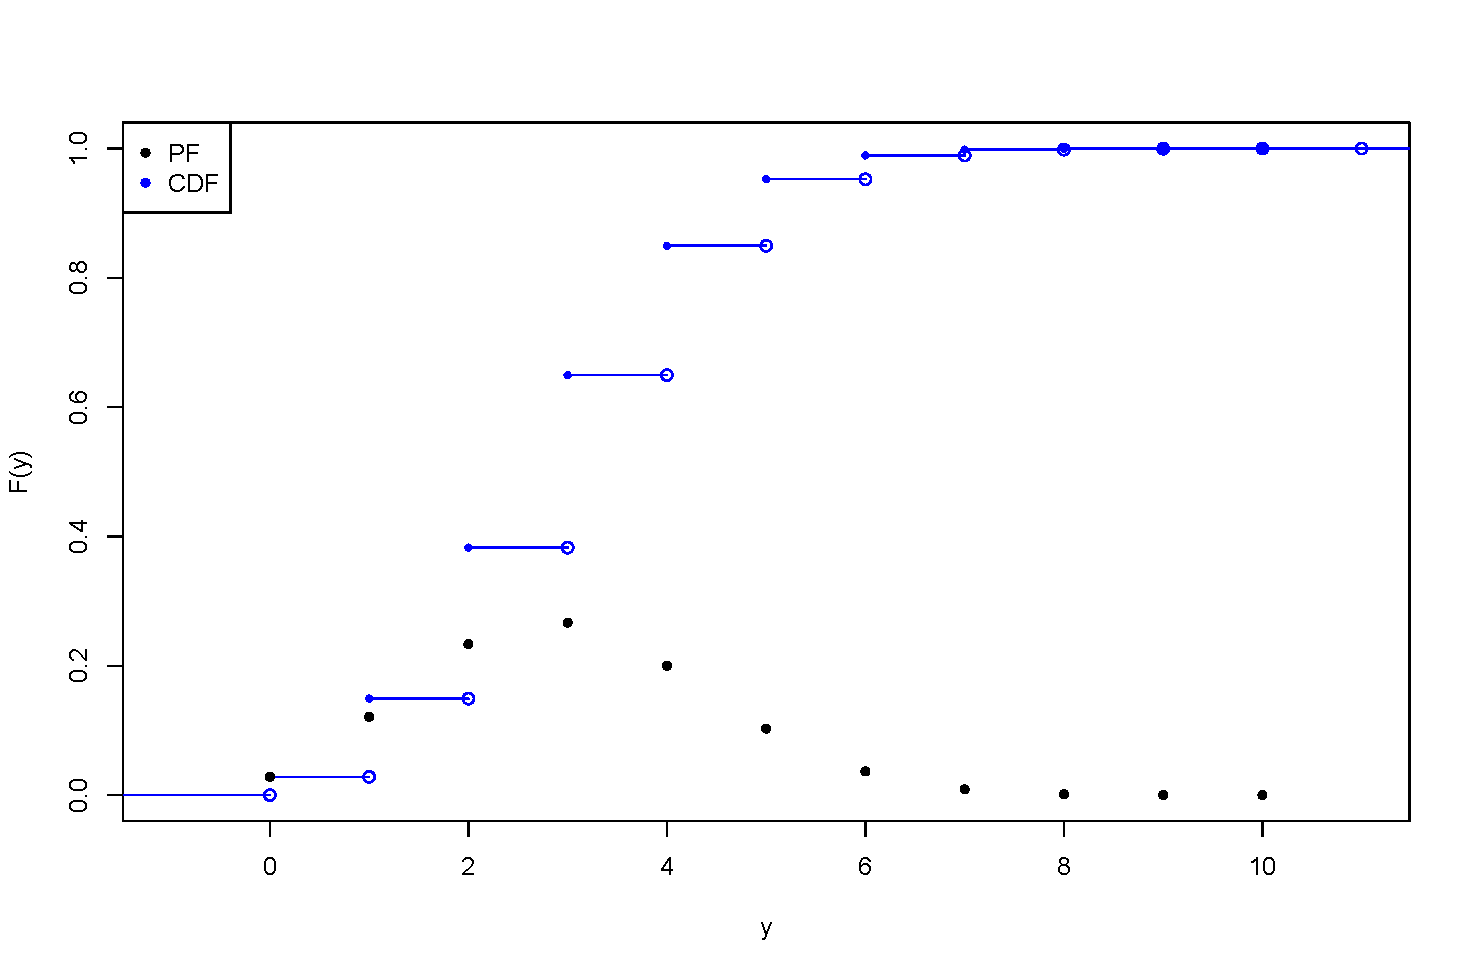
\includegraphics[width=4 in]{bindists.pdf}


\end{frame}


\begin{frame}
\frametitle{Functions of Random Variables}
We might (or often) apply a function to a random variable $g(X)$. \pause  \\
How do we compute $E[g(X)]$? \pause \\

\begin{prop}  \pause 
Expected value of a function of a random variable: Suppose $X$ is a discrete random variable that takes on values $x_{i}$, $i=\{1, 2, \hdots, $, with probabilities $p(x_{i})$. \pause  If $g:X \rightarrow \mathcal{R}$, then its expected value $E[g(X)]$ is, \pause 
\begin{eqnarray}
E[g(X)] & = & \sum_{i} g(x_{i}) p(x_{i} ) \nonumber 
\end{eqnarray}
\end{prop}

\end{frame}

\begin{frame}
\frametitle{Functions of Random Variables: Corollary} 



\begin{cor}
Suppose $X$ is a random variable and $a$ and $b$ are \alert{constants} (not random variables).  Then, 
\begin{eqnarray}
E[aX + b] & = & aE[X] + b \nonumber 
\end{eqnarray}
\end{cor}
\pause 
\begin{proof} 
\begin{eqnarray}
E[aX + b]  & = & \sum_{x: p(x)>0} (a x + b)p(x) \nonumber \\ \pause 
& = & \sum_{x:p(x)>0} a x p(x) + \sum_{x:p(x)>0} b p(x) \nonumber \\ \pause 
& = & a \sum_{x:p(x)>0} x p(x) + b \sum_{x:p(x)>0} p(x) \nonumber \\ \pause 
& = & a E[X] + b (1) \nonumber 
 \end{eqnarray}
 \end{proof} 


\end{frame}




\begin{frame}
\frametitle{Famous Distributions}

\begin{itemize}
\item[-] Bernoulli (coin flips)
\item[-] Binomial (sums of coin flips)
\item[-] Multinomial (multivariate coin flips)
\item[-] Poisson (sums of events over time or space)
\end{itemize}

\alert{Models} of how world works.  


\end{frame}



\begin{frame}
\frametitle{Poisson Distribution}

\begin{defn}
Suppose $X$ is a random variable that takes on values $X \in \{0, 1, 2, \hdots, \}$ and that $P(X = k) = p(k)$ is,
\begin{eqnarray}
p(k) & = & e^{-\lambda} \frac{\lambda^{k}}{k!} \nonumber 
\end{eqnarray}
for $k \in \{0, 1, \hdots, \}$ and $0$ otherwise.  Then we will say that $X$ follows a \alert{Poisson} distribution with \alert{rate} parameter $\lambda$.  \\
\begin{eqnarray}
X & \sim & \text{Poisson}(\lambda) \nonumber 
\end{eqnarray}

\end{defn}




\end{frame}






\begin{frame}
\frametitle{Poisson Distribution}
Properties:
\begin{itemize}
\item[1)] It is a probability distribution. \\
\item Recall the \alert{Taylor expansion} of $e^{x}$
\begin{eqnarray}
e^{x} & = & 1 + x + \frac{x^{2}}{2!} + \frac{x^3}{3!} + \hdots \nonumber \pause 
\end{eqnarray}
\item Now expand the pdf of the poisson distribution:
\begin{eqnarray}
e^{-\lambda} \sum_{k=0}^{\infty} \frac{\lambda^{k} }{k!} & = & e^{-\lambda}(1 + \lambda  + \frac{\lambda^2}{2!} + \hdots ) \nonumber  \pause\\
 & = & e^{-\lambda} (e^{\lambda}) = 1 \nonumber 
\end{eqnarray}
\end{itemize}

\end{frame}

\begin{frame}
\frametitle{Poisson Distribution}

\begin{itemize}
\item[2)] $E[X] = \lambda$, that is, the parameter of the poisson distribution is its expectation
\end{itemize}
\begin{eqnarray}
E[X] & = & e^{-\lambda} \sum_{k=0}^{\infty} k \frac{\lambda^{k}}{k!} \nonumber \\
& = & e^{-\lambda} \lambda \sum_{k=1}^{\infty} \frac{\lambda^{k-1}}{(k-1)!} \nonumber \pause
\end{eqnarray}
Define $j = k-1$, then 
\begin{eqnarray}
E[X]  & = & e^{-\lambda} \lambda \sum_{j=0}^{\infty} \frac{\lambda^{j}}{j!} \nonumber \pause\\
& = & e^{-\lambda} \lambda e^{\lambda} \nonumber \pause\\
& = & \lambda \nonumber 
\end{eqnarray}



\end{frame}

\begin{frame}
\frametitle{Poisson Distribution}
Properties:

\begin{itemize}
\item[3)] var$(X) = \lambda$\pause
\end{itemize}

\begin{eqnarray}
E[X^2] & = & \sum_{k=0}^{\infty} \frac{k^2 e^{-\lambda} \lambda^{k}}{k!} \nonumber \pause\\
& = & \lambda e^{-\lambda} \left(\sum_{k=1}^{\infty} \frac{k \lambda^{k-1}}{(k-1)!}\right)\nonumber \pause
\end{eqnarray}
Let $j = k-1$,\pause
\begin{eqnarray}
E[X^2] & = & \lambda e^{-\lambda} \sum_{j=0}^{\infty} \frac{(j+1) \lambda^{j}}{j!} \nonumber \pause \\
& = & \lambda e^{-\lambda} \left(\sum_{j=0}^{\infty} \frac{(j) \lambda^{j}}{j!} + \sum_{j=0}^{\infty} \frac{(1) \lambda^{j}}{j!} \right) \nonumber \pause \\
& = & \lambda e^{-\lambda} (\lambda e^{\lambda} + e^{\lambda} ) \nonumber \\
\end{eqnarray}


\end{frame}

\begin{frame}

\frametitle{Poisson Distribution}
Properties
\begin{itemize}
\item[3)] var$(X) = \lambda$
\end{itemize}

\begin{eqnarray}
E[X^2] & = & \lambda e^{-\lambda} (\lambda e^{\lambda} + e^{\lambda} ) \nonumber \pause \\
& = & \lambda (\lambda  + 1 ) \nonumber 
\end{eqnarray}


var$(X) = E[X^2] - E[X]^2 = \lambda^2 + \lambda  - \lambda^2  = \lambda$





\end{frame}



\begin{frame}{Joint PMFs}
If we have more than one random variable, we can study their joint behavior.

If $(x,y)$ are possible values of random variables $X$ and $Y$, then 

$$p_{X,Y}(x, y)=P(X=x,\ Y=y)$$

\end{frame}

\begin{frame}{Joint PMFs}
If we have more than one random variable, we can study their joint behavior.

If $(x,y)$ are possible values of random variables $X$ and $Y$, then 

$$p_{X,Y}(x, y)=P(X=x \cap Y=y)$$

\end{frame}

\begin{frame}{Joint PMFs}
If we want to know the probability of a set of joint events $(x, y) \in A$
$$P((X,Y)\in A)=\sum_{(x,\ y)\in A} p_{X,Y} (x,\ y)$$
We can also calculate the pmfs of X and Y individually (these are the marginal distributions:

$$p_X(x)=\sum_y p_{X,Y}(x, y), \ \ \quad p_Y(y)=\sum_x p_{X,Y}(x, y)$$

\end{frame}



\begin{frame}{Example of Joint PMF}
$$\Omega_1=\{\text{Non-Democracy, \ \ Democracy}\}$$
$$X(\omega)=\begin{cases}
 0\text{ if $\omega=$Non-Democracy}\\
1\text{ if $\omega=$Democracy}
\end{cases}$$
\pause
$$\Omega_2=\{\text{not-Killed, \ \ Killed}\}$$
$$Y(\omega)=\begin{cases}
y= 0\text{ if $\omega=$not Killed}\\
y=1\text{ if $\omega=$Killed}
\end{cases}$$

\pause
\begin{table}
\begin{tabular}{lll|l}
		$p_{X,Y}$& 0& 1&$p_{Y}$\\
1 & 0.034& 0.005& 0.039\\
0 & 0.466 &0.495&  0.961\\
\hline
$p_{X}$& 0.5 &0.5&  1
\end{tabular}
\end{table}
\end{frame}


\begin{frame}
\frametitle{Linearity}
$$E[X+Y]=E[X]+E[Y]$$
Proof:
$$E[X+Y] = \sum_{x} \sum_{y} (x+y) p(x, y) $$  \pause 
$$=  \sum_{x} \sum_{y} x p(x, y )+ \sum_{x} \sum_{y} y p(x, y) $$  \pause 
$$=  \sum_{x} x \sum_{y} p(x, y )+  \sum_{y} y \sum_{x} p(x, y) $$  \pause 
$$=  \sum_{x} x p(x )+  \sum_{y} y p( y) $$  \pause 

\end{frame}



\begin{frame}
\frametitle{Conditional Probability Distribution Function}


\begin{defn}
Suppose $X$ and $Y$ are discrete random variables with joint pdf $p(x,y)$.  Then define the \alert{conditional probability function} $p(x|y)$ as 

\begin{eqnarray}
p(x|y) & = & \frac{p(x, y) }{p_{Y}(y) } \nonumber 
\end{eqnarray}

\end{defn}

\end{frame}


\begin{frame}
\frametitle{Why Does Marginalization Work?}

Begin with \alert{discrete} case. \pause 

Consider jointly distributed discrete random variables, $X$ and $Y$.  We'll suppose they have joint pmf,  \pause 
\begin{eqnarray}
\invisible<1-2>{P(X =x, Y = y) = p(x, y)\nonumber} \pause 
\end{eqnarray}
\invisible<1-3>{Suppose that the distribution allocates its mass at $x_{1}, x_{2}, \hdots, x_{M}$ and $y_{1}, y_{2}, \hdots, y_{N}$.  \\} \pause 


\invisible<1-4>{Define the conditional mass function $P(X= x| Y= y)$ as, } \pause 
\begin{eqnarray}
\invisible<1-5>{P(X=x|Y=y) \equiv & = & p(x|y) \nonumber} \pause  \\
\invisible<1-6>{& = & p(x,y)/p(y) \nonumber } \pause 
\end{eqnarray}


\invisible<1-7>{Then it follows that: } \pause 
\begin{eqnarray}
\invisible<1-8>{p(x,y)  & = & p(x|y)p(y) \nonumber } \pause 
\end{eqnarray}

\invisible<1-9>{Marginalizing \alert{over} $y$ to get $p(x)$ is then,} \pause 
\begin{eqnarray}
\invisible<1-10>{p(x_{j})  & =& \sum_{i=1}^{N} p(x_{j} |y_{i})p(y_{i} ) \nonumber } 
\end{eqnarray}

\end{frame}


\begin{frame}
\frametitle{A Table} 

\only<1>{\begin{tabular}{c|cc|c}
& Y = 0 & Y = 1 \\
\hline
X = 0 & p(0,0)  & p(0, 1) & p$_{X}$(0)\\
X = 1 & p(1,0) & p(1,1)  & p$_{X}$(1)\\
\hline
			& p$_{Y}$ (0) & p$_{Y}$ (1) 
\end{tabular}}


\only<2->{\begin{tabular}{c|cc|c}
& Y = 0 & Y = 1 \\
\hline 
X = 0 & 0.01 & 0.05 & ? \\
X = 1 & 0.25 & 0.69 & ? \\
\hline
& 0.26 & 0.74 & \\
\end{tabular}
}

\begin{eqnarray}
p_{X}(0) & = & p(0|y = 0) p(y= 0) + p(0|y=1) p(y=1) \nonumber \\ \pause
& = & \frac{0.01}{0.26} \times 0.26 + \frac{0.05}{0.74} \times 0.74 \nonumber \\\pause
& = & 0.06 \nonumber \pause
\end{eqnarray}

\begin{eqnarray}
p_{X}(1) & = & p(1|y = 0) p(y= 0) + p(1|y=1) p(y=1) \nonumber \\\pause
& = & \frac{0.25}{0.26} \times 0.26 + \frac{0.69}{0.74} \times 0.74 \nonumber \\\pause
& = & 0.94\nonumber 
\end{eqnarray}



\end{frame}


\begin{frame}

\begin{defn} 
Two random variables $X$ and $Y$ are independent if for any two sets of real numbers $A$ and $B$, \pause 
\begin{eqnarray}
P\{ X \in A , Y \in B \} & = & P\{X \in A\} P\{Y \in B\} \nonumber \pause  
\end{eqnarray}

Equivalently we will say $X$ and $Y$ are independent if,  \pause 
\begin{eqnarray}
p(x,y) & = & p_{X}(x) p_{Y}(y) \nonumber  \pause 
\end{eqnarray}

If $X$ and $Y$ are not independent, we will say they are \alert{dependent} 

\end{defn}

\end{frame}

\begin{frame}
\frametitle{Conditional Distribution}

If $X$ and $Y$ are independent, then 
\begin{eqnarray}
p_{X|Y} (x|y) & = & \frac{p(x,y)}{p_{Y}(y)} \nonumber \\
& = & \frac{p_{X}(x)p_{Y}(y)}{p_{Y}(y) }\nonumber \\
& = & p_{X}(x) \nonumber 
\end{eqnarray}

In words: the distribution of $X$ does not change as levels of $Y$ change.  

\end{frame}

\begin{frame}
\frametitle{Conditional Expectation}
$$\mathbb{E}(Y|X)=\sum_y y\cdot p_{Y|X} (y|x) $$
$\mathbb{E}(Y|X)$ is the \emph{best} way to predict Y given X.

\end{frame}









\begin{frame}
\frametitle{Continuous Random Variables}
Many times we deal with continuous events:
\begin{itemize}
\item Growth rate of an economy.\pause
\item Length of a recession.\pause
\item Where a ball goes through a soccer net.
\end{itemize}
\pause
We will need continuous random variables to assign numbers to these events.
\end{frame}




\begin{frame}
\frametitle{Probability of a continuous random variable}

\begin{defn}
If X is a continuous random variable, the probability density function of X is the function $f_X(x)$ that satisfies.
$$F_X(x)=P(X\leq x)$$\pause
$$=P(X\in (-\infty,\ x))$$
$$=\int_{-\infty}^{x} f_X(t)dt\ \ \ \ x\in \textbf{R}$$
\end{defn}
\pause
$$\int_a^b f_X(x)dx=P(X\in(a,b))$$
\end{frame}


\begin{frame}
\frametitle{Cumulative Distribution Function} 

Cumulative distribution functions fully characterize continuous random variables.\pause

\invisible<1>{\begin{defn} 
Cumulative Distribution function.  For a continuous random variable $X$ define its cumulative distribution function $F(\cdot )$ as, 
\begin{eqnarray} 
F(t) & = & P(X \leq t) = \int_{-\infty} ^{t} f(x) dx \nonumber 
\end{eqnarray}
\end{defn}} 
\pause 

\begin{center}
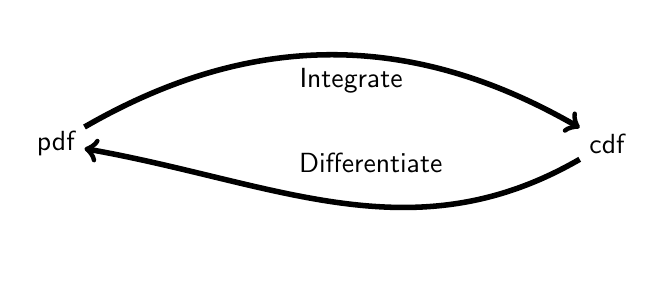
\begin{tikzpicture} 
\node (d1) at (-4, 3) [] {pdf};  
\node (f1) at (3, 3) [] {cdf} ; 
\draw[->, line width=2pt] (d1) to [out=30, in=150] (f1) ; 
\node (d2) at (-0.25, 3.8) [] {Integrate} ; 

\node (f2) at (0, 2.75) [] {Differentiate} ; 


\draw[->, line width=2pt] (f1) to [out=210, in=350] (d1); 
\end{tikzpicture}
\end{center}




\end{frame}




\begin{frame}
\frametitle{RV: continuous uniform}

\begin{defn}
We can define Y to have a uniform distribution on the interval $(a,b)$
$$f_Y(y)=\begin{cases} \frac{1}{b-a}& \text{if } a<y<b\\ 0 & \text{otherwise} \end{cases}$$
\end{defn}

\end{frame}
\begin{frame}{Example: Uniform}

Example: Suppose that we are waiting for Comcast to show up and install our cable package.  They say that they may arrive between 2:00 and 8:00.  Without any further information, you may have no reason to suspect any particular time over any other.
$$X\sim U(2,8)$$

\end{frame}





\begin{frame}
\frametitle{RV: continuous uniform}

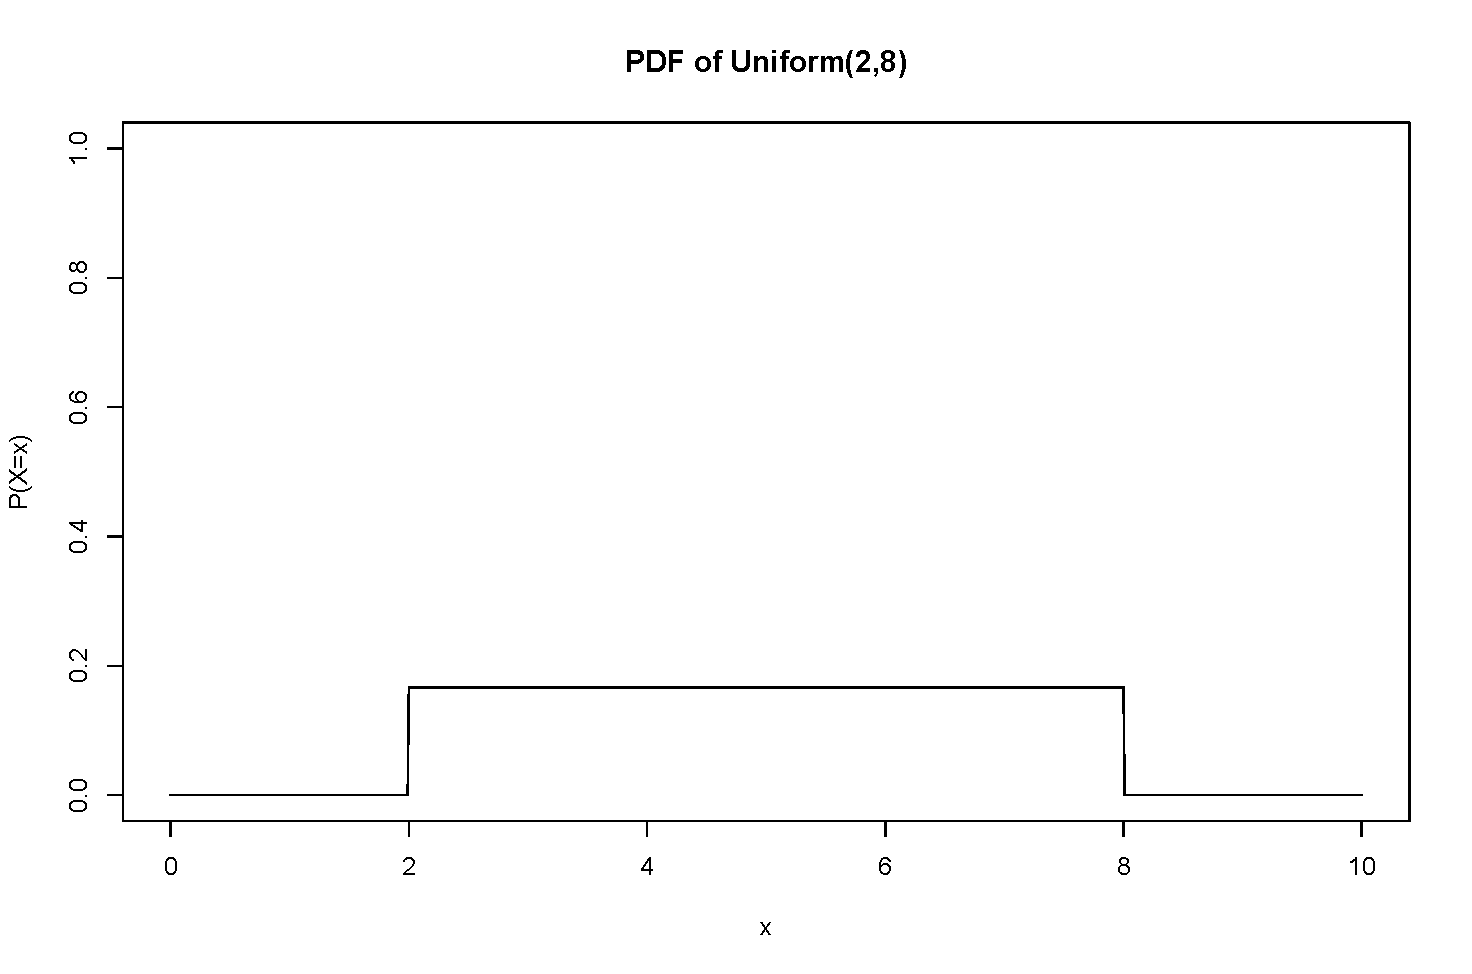
\includegraphics[width=4 in]{Udists2.pdf}


\end{frame}




\begin{frame}
\frametitle{RV: continuous uniform }
What is the probability that the cable installation truck arrives before 4:00?

\end{frame}


\begin{frame}
\frametitle{RV: continuous uniform ($P(X\leq4)$)}

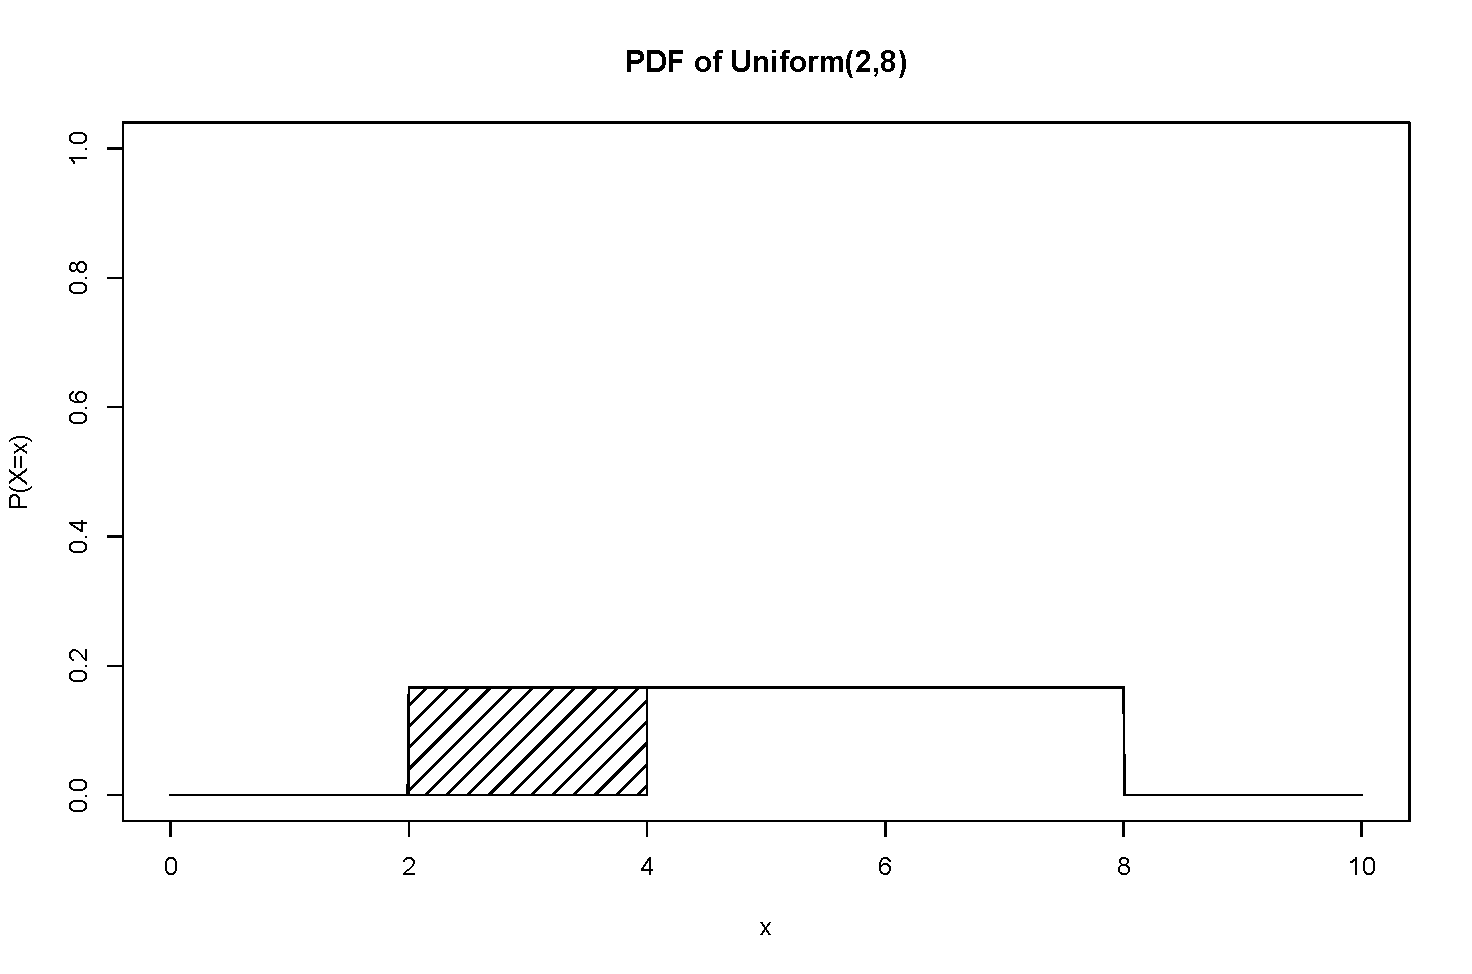
\includegraphics[width=3.5in]{Udists3.pdf}


\end{frame}




\begin{frame}
\frametitle{RV: continuous uniform}

$$P(Y\leq y)=\int_{x=-\infty}^{y}f(x)dx=\int_{x=-\infty}^{y}\frac{1}{b-a}dx=\int_{x=a}^{y}\frac{1}{b-a}dx$$\pause
$$\frac{y}{b-a}-\frac{a}{b-a}=\frac{y-a}{b-a}$$\pause
 $$=\frac{4-2}{8-2}$$

\end{frame}



\begin{frame}
\frametitle{RV: continuous uniform}

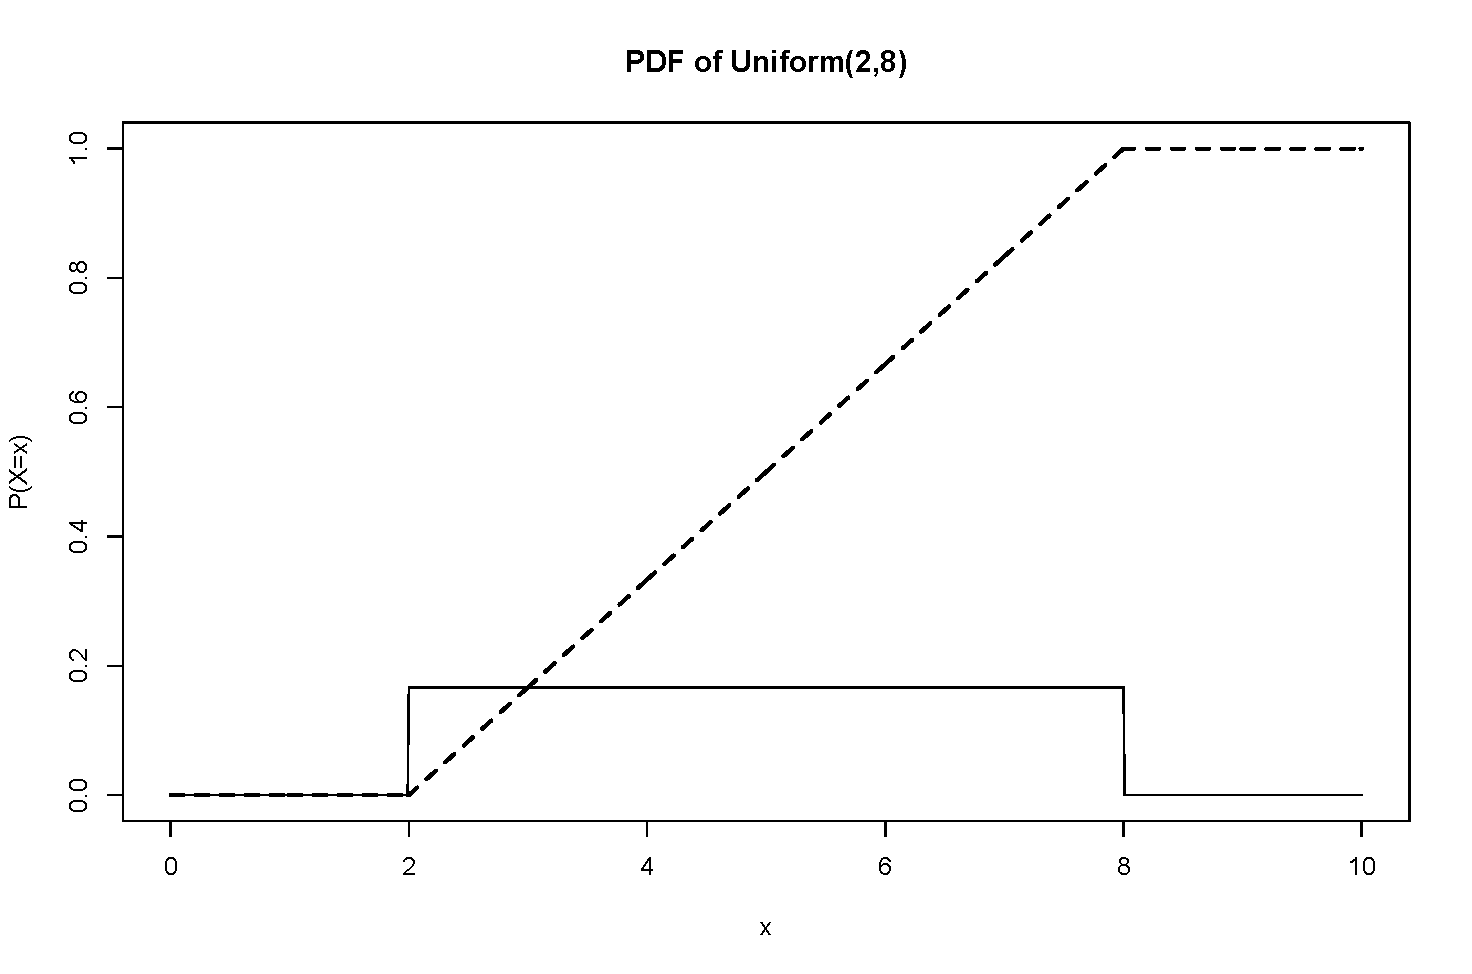
\includegraphics[width=3.5 in]{Udists4.pdf}


\end{frame}

\begin{frame}
\frametitle{Common Continuous Distributions: Exponential}

Example: Suppose that the average durability of a Peace Accord in the Democratic Republic of Congo is 6 months. How can we model the time to failure of Peace Accord?\pause

The exponential distribution is often used to model `time to failure' processes.\pause

$X\sim \exp(\lambda)$ if its PDF is:
$$f(x)=\lambda e^{-\lambda x}$$
with $f(x)=0$ for $x<0$\pause

$\lambda$ is known as the 'rate' parameter.

$\lambda=\frac{1}{E(X)}$
\end{frame}


\begin{frame}
\frametitle{Exponential CDF}
The CDF of $X\sim\exp(\lambda)$ is:

$$F(x)= \int_{-\infty}^x f(x)dx=\int_{0}^x \lambda e^{-\lambda x}dx$$\pause
$$= F(x)-F(0)$$\pause
where F(x) is the antiderivative of f(x).\pause
$$= - \frac{\lambda e^{-\lambda x}}{\lambda} - (- \frac{\lambda e^{-\lambda*0}}{\lambda})$$\pause
$$=1-e^{-\lambda x}$$
\end{frame}



\begin{frame}
\frametitle{Expectation With Continuous Random Variables} 

\begin{defn} 
If $X$ is a continuous random variable then, 
\begin{eqnarray}
E[X] & = & \int_{-\infty}^{\infty} x f(x) dx \nonumber 
\end{eqnarray}
\end{defn} 


\end{frame}


\begin{frame}
Suppose $X \sim Uniform(0,1)$.  What is $E[X]$? \pause 
\begin{eqnarray}
E[X] \pause & = & \int_{-\infty}^{\infty} xf(x)dx \nonumber  \pause \\
& = & \int_{-\infty}^{0} x 0 dx + \int_{0}^{1} x 1 dx + \int_{1}^{\infty} x 0 dx \nonumber \pause  \\
& = & 0 +  \frac{x^{2}}{2} |^{1}_{0} + 0 \nonumber  \pause \\
& = & 0 + \frac{1}{2} + 0 \nonumber \pause \\
& = & \frac{1}{2} \nonumber 
\end{eqnarray}


\end{frame}


\begin{frame}
\frametitle{Expectations of Functions} 
\begin{prop} 
Suppose $X$ is a continuous random variable and $g:\Re \rightarrow \Re$.  Then, 
\begin{eqnarray}
E[g(X)] & = & \int_{-\infty}^{\infty} g(x)f(x)dx \nonumber 
\end{eqnarray}
\end{prop} 

\end{frame}


\begin{frame}
\frametitle{Expectations of Functions} 

Suppose $g(X) = X^2$  and $X \sim \text{Uniform}(0,1)$.  What is E[g(X)]? \pause 

\begin{eqnarray}
E[g(X)] \pause  & = & \int_{-\infty}^{\infty} g(x)f(x)dx \nonumber \pause  \\
& = & \int_{0}^{1} x^2 \frac{1}{1-0}dx \nonumber  \pause \\
& = & \frac{x^3}{3}|^{1}_{0} \nonumber  \pause \\
& = & \frac{1}{3} \nonumber 
\end{eqnarray}


\end{frame}


\begin{frame}

\begin{cor} 
Suppose $X$ is a continuous random variable.  Then, 
\begin{eqnarray}
E[aX + b] & = & aE[X] + b\nonumber 
\end{eqnarray}
\end{cor}
\pause 

\begin{proof}
\begin{eqnarray}
E[aX + b] & = & \int_{-\infty}^{\infty} (a x + b)f(x) dx \nonumber \\ \pause 
& = & a \int_{-\infty}^{\infty} x f(x) dx + b \int_{-\infty}^{\infty} f(x)dx \nonumber \\ \pause 
& = & a E[X]  + b \times 1 \nonumber 
\end{eqnarray}


\end{proof}


\end{frame}




\begin{frame}


\begin{defn} 
Variance.  If $X$ is a continuous random variable, define its variance, $Var(X)$, 
\begin{eqnarray}
Var(X) & = & E[(X- E[X])^2] \nonumber \\
& = & \int_{-\infty}^{\infty} (x - E[X])^2f(x) dx \nonumber \\
& = & E[X^2] - E[X]^2 \nonumber 
\end{eqnarray}
\end{defn}

\end{frame}



\begin{frame}
\frametitle{Variance: Random Variable} 

$X \sim \text{Uniform}(0,1)$.  What is $Var(X)$? \pause   

\begin{eqnarray} 
E[X^2] & = & \frac{1}{3} \nonumber  \pause \\
E[X]^2 & = & \left(\frac{1}{2}\right)^2 \nonumber \pause \\
& = & \frac{1}{4} \nonumber \pause  
\end{eqnarray}

\begin{eqnarray}
Var(X) & =& E[X^2] - E[X]^2  \pause \nonumber \\
& = &  \frac{1}{3} - \frac{1}{4} = \alert{\frac{1}{12}} \nonumber 
\end{eqnarray}

\end{frame}



\begin{frame}

\begin{defn}
Suppose $X$ is a random variable with $X \in \mathbf{R}$ and probability density function

\begin{eqnarray}
f(x) & = & \frac{1}{\sqrt{2\sigma^2\pi}}\exp\left(-\frac{(x - \mu)^2}{2\sigma^2}\right) \nonumber 
\end{eqnarray}

Then $X$ is a \alert{normally} distributed random variable with parameters $\mu$ and $\sigma^2$.  \\


Equivalently, we'll write 
\begin{eqnarray}
X & \sim & \text{Normal}(\mu, \sigma^2) \nonumber 
\end{eqnarray}




\end{defn}
\end{frame}



\begin{frame}
\frametitle{Support for President Trump} 

Suppose we are interested in modeling \alert{presidential approval} \pause 
\begin{itemize}
\item[-] Let $Y$ represent random variable: proportion of population who ``approves job president is doing" \pause 
\item[-] Individual responses (that constitute proportion) are \alert{independent} and \alert{identically} distributed (sufficient, not necessary) and we take the average of those individual responses \pause 
\item[-] Observe \alert{many} responses ($N\rightarrow \infty$) \pause 
\item[-] Then (by Central Limit Theorem) $Y$ is \alert{Normally} distributed, or  \pause 
\end{itemize}
\begin{eqnarray}
Y& \sim & \text{Normal}(\mu, \sigma^2) \nonumber  \pause \\
f(y) & = & \frac{\exp\left(-\frac{(y-\mu)^2}{2\sigma^2} \right)}{\sqrt{2\pi \sigma^2}} \nonumber 
%\text{Mean} & = & \alert{\mu} \nonumber \\
%\text{Variance} & = & \alert{\sigma^2} \nonumber  
\end{eqnarray}

\end{frame}



\begin{frame}
\frametitle{Expected Value/Variance of Normal Distribution}

$Z$ is a standard normal distribution if \pause 
\invisible<1>{\begin{eqnarray}
Z & \sim & \text{Normal}(0,1) \nonumber 
\end{eqnarray}
} \pause 



\invisible<1-2>{We'll call the cumulative density function of $Z$, } \pause 
\begin{eqnarray}
F_{Z}(x) & = & \frac{1}{\sqrt{2\pi} }\int_{-\infty}^{x} \exp(-z^2/2) dz \nonumber  \pause 
\end{eqnarray}


\begin{prop} 
\alert{Scale/Location}.  If $Z \sim N(0,1)$, then $X = aZ + b$ is, 
\begin{eqnarray}
X & \sim & \text{Normal} (b, a^2) \nonumber 
\end{eqnarray}
\end{prop}



\end{frame}




\begin{frame}
\frametitle{Proof:$Z \sim N(0,1)$ and $Y = aZ + b$, then  $Y \sim N(b, a^2)$ } 
To prove\pause  we need to show that density for $Y$ is a normal distribution.  \pause  \\
That is, we'll show $F_{Y}(x)$ is Normal cdf.\pause   \\
Call $F_{Z}(x)$ cdf for standardized normal. \pause   

\begin{eqnarray}
F_{Y} (x) & = & P(Y \leq x) \nonumber  \pause  \\
& = & P(aZ + b \leq x) \nonumber  \pause  \\
& = & P(Z \leq \left[\frac{x - b}{a} \right] ) \nonumber  \pause  \\
& = & \frac{1}{\sqrt{2\pi} } \int_{-\infty}^{\frac{x-b}{a} } \exp( - \frac{z^2}{2} ) dz \nonumber \pause  \\
& = &F_{Z} (\frac{x - b}{a} )\nonumber 
 \end{eqnarray}
\end{frame}


\begin{frame}
\frametitle{Proof:$Z \sim N(0,1)$ and $Y = aZ + b$, then  $Y \sim N(b, a^2)$ } 

So, we can work with $F_{Z}(\frac{x - b}{a} )$.  \pause 
\begin{eqnarray}
\frac{\partial F_{Y}(x) }{\partial x} & =& \frac{\partial F_{Z} (\frac{x - b}{a} ) }{\partial x} \nonumber \pause \\
& = & f_{Z} (\frac{x - b}{a} ) \frac{1}{a}  \text{ By the chain rule } \pause \nonumber \\
& = & \frac{1}{\sqrt{2 \pi } a } \exp\left[-\frac{\left(\frac{x-b}{a} \right)^2}{2 }\right] \nonumber \text{ By definition of $f_{Z}(x)$ } \pause \\
& = & \frac{1}{\sqrt{2 \pi } a } \exp\left[-\frac{\left(x-b\right)^2}{2a^2 }\right] \nonumber  \pause \\
& = & \text{Normal} (b, a^2) \nonumber 
\end{eqnarray}

\end{frame}

\begin{frame}
\frametitle{Expectation and Variance}

Assume we know:
\begin{eqnarray}
E[Z]  & = & 0 \nonumber \\
Var(Z) & = & 1 \nonumber 
\end{eqnarray}
\pause 
This implies that, for $Y \sim \text{Normal}(\mu, \sigma^2)$ \pause 
\begin{eqnarray} 
E[Y] & = & E[\sigma Z + \mu] \nonumber  \pause \\
& = & \sigma E[Z] + \mu \nonumber  \pause \\
& = & \mu \nonumber \pause \\
Var(Y) & = & Var(\sigma Z + \mu) \nonumber \pause \\
& = & \sigma^2 Var(Z) + Var(\mu) \nonumber  \pause \\
& = & \sigma^2 + 0 \nonumber \pause \\
 & =& \sigma^2 \nonumber 
\end{eqnarray}

\end{frame}





\begin{frame}
\frametitle{Back To Trump} 

Suppose $\mu = 0.39$ and $\sigma^2 = 0.0025$ \pause  \\
$P(Y\geq 0.45)$  \pause 
\begin{eqnarray} 
P(Y \geq 0.45)  &  = & 1 - P(Y \leq 0.45 ) \nonumber \pause  \\
& = &  1 - P(0.05 Z + 0.39 \leq  0.45)   \nonumber  \pause\\
& = & 1 - P(Z \leq \frac{0.45-0.39 }{0.05} ) \nonumber \pause \\
& = & 1 - \frac{1}{\sqrt{2\pi} } \int_{-\infty}^{6/5} \exp(-z^2/2) dz \pause   \nonumber \\
& = & 1 - F_{Z} (\frac{6}{5} ) \nonumber \pause\\
& = & 0.1150697 \nonumber 
\end{eqnarray}
\end{frame}

\begin{frame}
\frametitle{The Gamma Function}

\begin{defn}
Suppose $\alpha>0$.  Then define $\Gamma(\alpha)$ as 
\begin{eqnarray}
\Gamma(\alpha) & = & \int_{0}^{\infty} y^{\alpha- 1} e^{-y} dy \nonumber 
\end{eqnarray}
\end{defn}

\begin{itemize}
\item[-] For $\alpha \in \{1, 2, 3, \hdots\}$\\
 $\Gamma(\alpha) = (\alpha- 1)!$
\item[-] $\Gamma(\frac{1}{2}) = \sqrt{\pi}$
\end{itemize}


\end{frame}


\begin{frame}
\frametitle{Gamma Distribution}

Suppose we have $\Gamma(\alpha)$,  \pause 
\begin{eqnarray}
\frac{\Gamma(\alpha)}{\Gamma(\alpha)} & = & \frac{\int_{0}^{\infty} y^{\alpha-1} e^{-y} dy}{\Gamma(\alpha)} \nonumber \\
1 & = & \int_{0}^{\infty} \frac{1}{\Gamma(\alpha)} y^{\alpha-1} e^{-y} dy \nonumber  \pause 
\end{eqnarray}

Set $X = Y/\beta$ \pause 

\begin{eqnarray}
F(x) = P(X \leq x) & = & P(Y/\beta \leq x ) \nonumber \pause\\
& = & P(Y \leq x \beta ) \nonumber \pause\\
 & = & F_{Y} (x \beta) \nonumber \pause\\
\frac{\partial F_{Y} (x \beta) }{\partial x} & = & f_{Y} (x \beta) \beta \nonumber 
\end{eqnarray}

The result is: \pause 
 \begin{eqnarray}
f(x|\alpha, \beta) & = & \frac{\beta^{\alpha}}{\Gamma(\alpha)} x^{\alpha - 1} e^{-x\beta}  \nonumber 
 \end{eqnarray}



\end{frame}


\begin{frame}

\begin{defn}
Suppose $X$ is a continuous random variable, with $X \geq 0$.  Then if the pdf of $X$ is 
 \begin{eqnarray}
f(x|\alpha, \beta) & = & \frac{\beta^{\alpha}}{\Gamma(\alpha)} x^{\alpha - 1} e^{-x\beta}  \nonumber 
 \end{eqnarray}

if $x\geq 0$ and $0$ otherwise, we will say $X$ is a Gamma distribution. 
\begin{eqnarray}
X & \sim & \text{Gamma}(\alpha, \beta) \nonumber 
\end{eqnarray}

\end{defn}


\end{frame}


\begin{frame}
\frametitle{Gamma Distribution}

Suppose $X \sim \text{Gamma}(\alpha, \beta)$ \pause 
\begin{eqnarray}
E[X] & = & \frac{\alpha}{\beta} \nonumber \pause\\
\text{var}(X) & = & \frac{\alpha}{\beta^2} \nonumber \pause\\
\end{eqnarray}



Suppose $\alpha = 1$ and $\beta = \lambda$.  If \pause\\
\begin{eqnarray}
X & \sim & \text{Gamma}(1, \lambda) \nonumber \pause\\
f(x|1, \lambda ) & = & \lambda e^{- x \lambda}  \nonumber
\end{eqnarray}



We will say \pause 
\begin{eqnarray}
X & \sim & \text{Exponential}(\lambda) \nonumber 
\end{eqnarray}


\end{frame}

\begin{frame}
\frametitle{Properties of Gamma Distributions}

\begin{prop}
Suppose we have a sequence of independent random variables, with 
\begin{eqnarray}
X_{i} & \sim & \text{Gamma}(\alpha_{i}, \beta) \nonumber 
\end{eqnarray}
Then 
\begin{eqnarray}
Y = \sum_{i=1}^{N} X_{i} \nonumber 
\end{eqnarray}

$Y \sim \text{Gamma}(\sum_{i=1}^{N} \alpha_{i} , \beta) $


\end{prop}


\end{frame}





\begin{frame}
We can evaluate in {\tt R} with {\tt dgamma} and simulate with {\tt rgamma}\\

$X \sim \text{Gamma}(3, 5)$ and we evaluate at 3, \\
{\tt dgamma(3, shape= 3, rate = 5)}\\
and we can simulate with \\
{\tt rgamma(1000, shape = 3, rate = 5)} 




\end{frame}


\begin{frame}

\begin{center}

\scalebox{0.5}{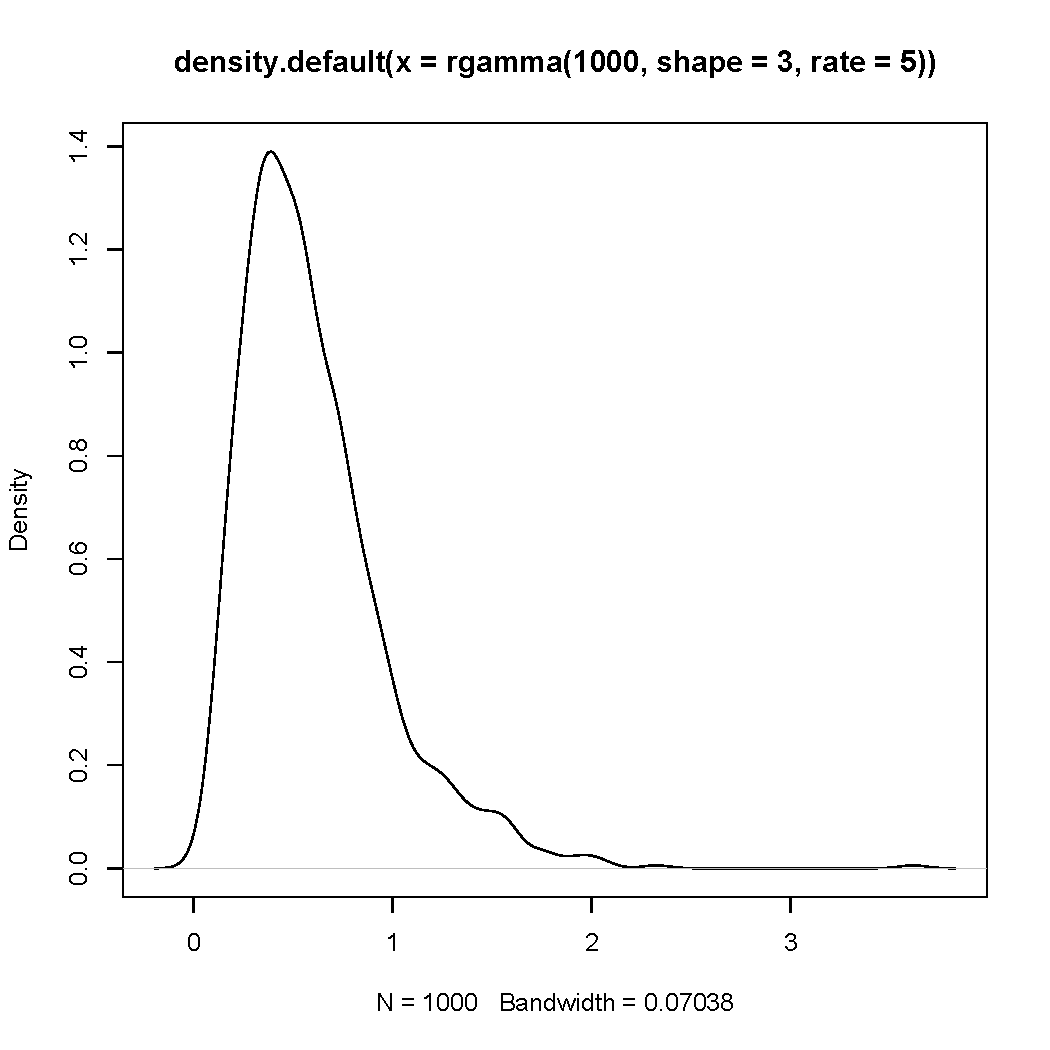
\includegraphics{GammaPlot.pdf}}

\end{center}

\end{frame}


\begin{frame}
\frametitle{$\chi^{2}$ Distribution}

Suppose $Z \sim \text{Normal}(0,1)$. \pause   \\
Consider $X = Z^2$ \pause 
\begin{eqnarray}
F_{X}(x)   & = &  P(X \leq x) \nonumber \\  \pause 
& = & P(Z^2 \leq x ) \nonumber \\ \pause 
& = & P(-\sqrt{x} \leq Z \leq \sqrt{x}) \nonumber \\ \pause 
& = & \frac{1}{\sqrt{2\pi}} \int_{-\sqrt{x}}^{\sqrt{x} } e^{-\frac{z^2}{2}} dz \nonumber \\ \pause 
& = & F_{Z} (\sqrt{x}) - F_{Z} (-\sqrt{x}) \nonumber 
\end{eqnarray}
\invisible<1-7>{The pdf then is } \pause 

\begin{eqnarray}
\frac{\partial F_{X}(x) }{\partial x }  & = & f_{Z} (\sqrt{x}) \frac{1}{2\sqrt{x}} + f_{Z}(-\sqrt{x}) \frac{1}{2\sqrt{x}} \nonumber  
\end{eqnarray}

\pause 




\end{frame}

\begin{frame}
\frametitle{$\chi^2$ Distribution}
\begin{eqnarray}
\frac{\partial F_{X}(x) }{\partial x }  & = & f_{Z} (\sqrt{x}) \frac{1}{2\sqrt{x}} + f_{Z}(-\sqrt{x}) \frac{1}{2\sqrt{x}} \nonumber \pause \\
& = & \frac{1}{\sqrt{x}}\frac{1}{2 \sqrt{2\pi}} ( 2e^{-\frac{x}{2}}) \nonumber \\ \pause 
& = & \frac{1}{\sqrt{x}}\frac{1}{\sqrt{2\pi}} ( e^{-\frac{x}{2}}) \nonumber \\ \pause 
& = & \frac{(\frac{1}{2})^{1/2}}{\Gamma(\frac{1}{2})}\left(x^{1/2 - 1} e^{-\frac{x}{2}}\right) \nonumber \pause 
\end{eqnarray}

$X \sim \text{Gamma}(1/2, 1/2)$\pause 

Then if $X = \sum_{i=1}^{N} Z^2$\\  \pause 

$X \sim \text{Gamma}(n/2, 1/2) $



\end{frame}


\begin{frame}

\begin{defn}
Suppose $X$ is a continuous random variable with $X\geq 0$, with pdf 

\begin{eqnarray}
f(x) & = & \frac{1}{2^{n/2} \Gamma(n/2) } x^{n/2 - 1} e^{-x/2} \nonumber 
\end{eqnarray}

Then we will say $X$ is a $\chi^2$ distribution with $n$ degrees of freedom.  Equivalently,

\begin{eqnarray}
X & \sim & \chi^{2}(n) \nonumber 
\end{eqnarray}

\end{defn}



\end{frame}


\begin{frame}
\frametitle{$\chi^2$ Properties}

Suppose $X \sim \chi^2(n)$
\begin{eqnarray}
E[X] & = & E\left[\sum_{i=1}^{N} Z_{i}^2\right] \nonumber \\
 & = & \sum_{i=1}^{N} E[Z_{i}^{2} ] \nonumber \\
\text{var}(Z_{i} ) & = & E[Z_{i}^2] - E[Z_{i}]^2 \nonumber\\
1 & = & E[Z_{i}^2]- 0 \nonumber \\
E[X] & = & n \nonumber 
 \end{eqnarray}



\end{frame}

\begin{frame}
\frametitle{$\chi^2$ Properties}

\begin{eqnarray}
\text{var}(X) & = & \sum_{i=1}^{N} \text{var}(Z_{i}^2) \nonumber \\
& = & \sum_{i=1}^{N} \left(E[Z_{i}^{4} ] - E[Z_{i}]^{2}  \right) \nonumber \\
& = & \sum_{i=1}^{N} \left(3 - 1\right ) = 2n \nonumber 
\end{eqnarray}

We will use the $\chi^2$ in all sorts of statistics courses  


\end{frame}


\begin{frame}
\frametitle{Student's $t$-Distribution}

\begin{defn}
Suppose $Z \sim \text{Normal}(0, 1)$ and $U \sim \chi^2(n)$.  Define the random variable $Y$ as, 

\begin{eqnarray}
Y & = & \frac{Z}{\sqrt{\frac{U}{n}}} \nonumber 
\end{eqnarray}

If $Z$ and $U$ are independent then $Y \sim t(n)$, with pdf 

\begin{eqnarray}
f(x) & = & \frac{\Gamma(\frac{n+1}{2})}{\sqrt{\pi n } \Gamma(\frac{n}{2})}\left(1 + \frac{x^2}{n}\right)^{-\frac{n+1}{2}} \nonumber 
\end{eqnarray}

We will use the t-distribution extensively for \alert{test-statistics}


\end{defn}

\end{frame}


\begin{frame}
\frametitle{Student's $t$-Distribution, Properties}

Suppose $n = 1$, \alert{Cauchy} distribution

\only<1>{\scalebox{0.25}{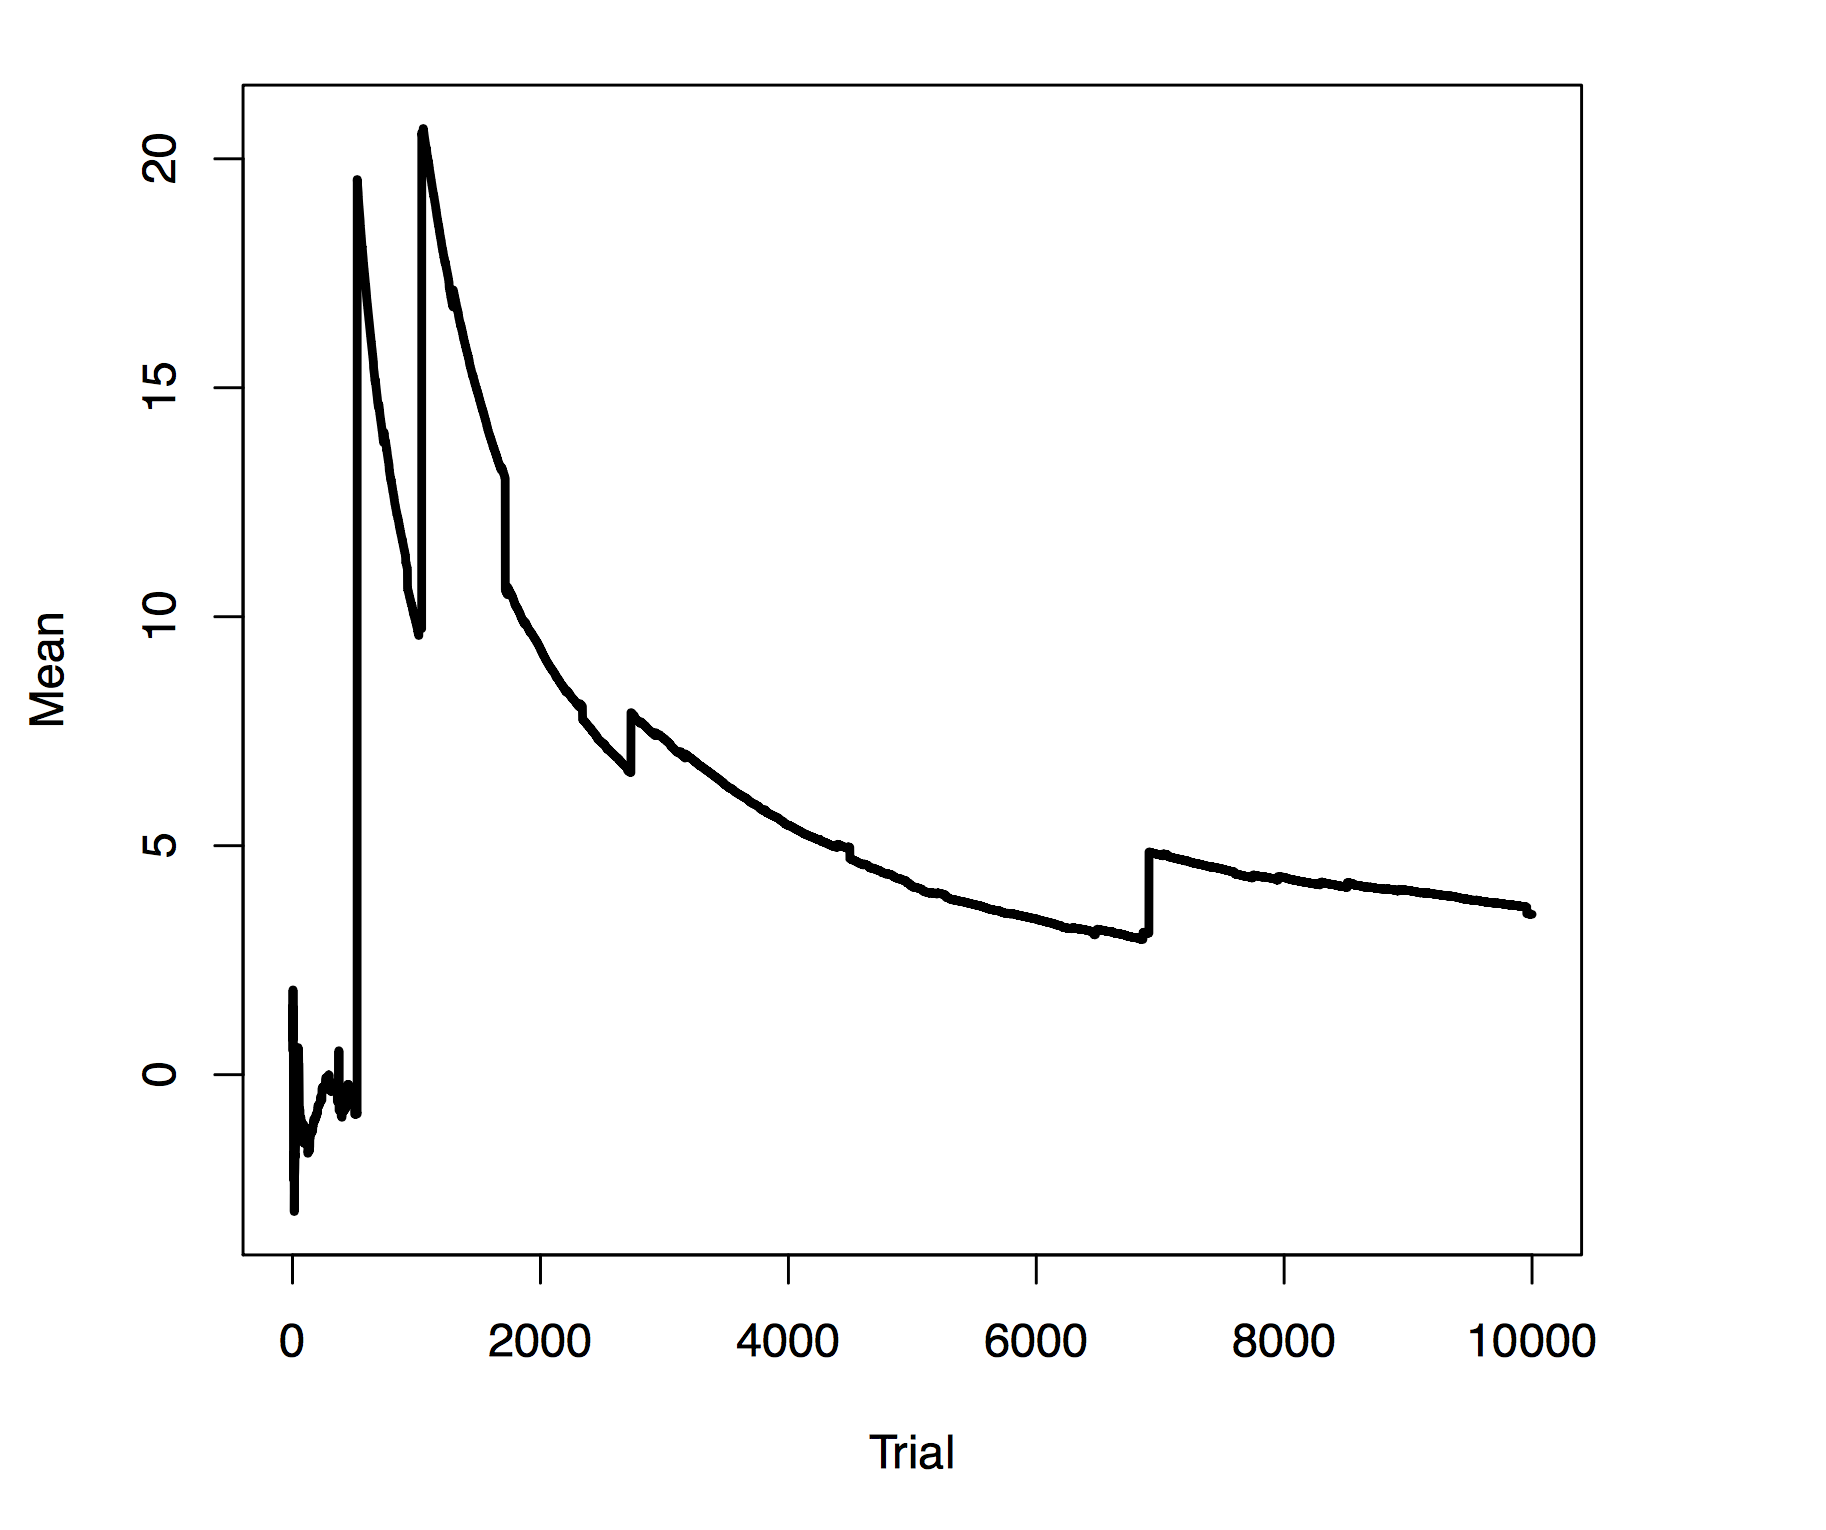
\includegraphics{Cauchy1.png}}} 
\only<2->{
If $X \sim \text{Cauchy}(1)$, then:\\
\invisible<1-2>{$E[X] =$ undefined \\} 
\invisible<1-3>{var$(X)$ = undefined \\} 

\invisible<1-4>{If $X \sim t(2)$ \\} 
\invisible<1-5>{E[X] = 0  \\} 
\invisible<1-6>{$\text{var}(X) $ = undefined} 

}


\pause \pause \pause \pause \pause \pause 

\end{frame}


\begin{frame}
\frametitle{Student's $t$-Distribution, Properties}

Suppose $n>2$, then \\
$var(X) = \frac{n}{n-2}$ \\
As $n \rightarrow \infty$ var$(X) \rightarrow 1$.  



\end{frame}



\begin{frame}
\frametitle{Using the t-Distribution}

We often construct \alert{test-statistics}\\
Suppose we take $N$ iid draws, 
\begin{eqnarray}
X_{i} & \sim & \text{Normal}(\mu, \sigma^2) \nonumber 
\end{eqnarray}

Define our data set $\boldsymbol{x} = (x_{1}, \hdots, x_{N})$

Calculate:
\begin{eqnarray}
 \bar{x} & = &  \sum_{i=1}^{N} \frac{x_{i}}{N} \nonumber \\
 s^2 & = & \frac{1}{N-1} \sum_{i=1}^{N} (x_{i} - \bar{x})^2 \nonumber 
\end{eqnarray}

\end{frame}

\begin{frame}
\frametitle{Estimators}
\begin{itemize}
\item Our data are realizations from a sample space.\pause
\item Functions of data are a kind of random variable called `statistics'. \pause  
\item If that function is used to infer the value of a parameter of a distribution, it is called an `estimator'.\pause
\item All estimators are statistics, and so they are random variables.\pause
\end{itemize}
$\bar{x}(X)$ is a function called the sample mean, and it produces estimates of the true mean ($\mu$)\\ \pause
$s^2(X)$ is a function called the sample variance, and it produces estimates of the true variance ($\sigma^2$).\\ \pause
Sometimes we will use little hats, to indicate that it is a function of a particular realization of the data.

\end{frame}
\begin{frame}
\frametitle{Estimators}
\begin{itemize}
\item Because estimators are random variables, they have a distribution.\pause
\item Our knowledge about the underlying world that produced our data is governed by these distributions.
\end{itemize}
\end{frame}

\begin{frame}
\frametitle{Using the T-Distribution}

Define 
\begin{eqnarray}
t & = & \frac{\bar{x} - \mu}{s/\sqrt{N}} \nonumber \\
t & \sim &Student's\ t(N-1) \nonumber 
\end{eqnarray}


\end{frame}




\end{document}
